\chapter{Automação de testes no desenvolvimento de uma aplicação}

\section{Contextualização da Aplicação}
Para realização da proposta deste trabalho, um ideia de protótipo foi gerada a partir de um Brainstorming, afim de criar uma aplicação para dispositivos móveis que fosse capaz de ajudar pessoas com deficiência auditiva ou surda, utilizando a tecnologia de classificação de sinais de áudio.

Segundo  o censo de 2010 do IBGE, 45.623.910 de pessoas, que equivalia a 23,9\% da população brasileira, declarou apresentar algum tipo de deficiência física. Sendo 9.722.163 de deficientes auditivos \cite{censo2010}. Um fator agravante desta realidade é a intensidade de sons que as pessoas estão submetidas ao decorrer do dia-a-dia. Alguns dos sons a seguir são exemplos que contribuem para a perda da audição: sons emitidos durante o tráfego de automóveis, obras em andamento, shows, boates e as músicas em volume exagerado nos fones de ouvido \cite{jornalDiaDia}. Segundo especialistas o limite saudável à exposição aos sons é de 80 decibéis (dB). Uma exposição diária acima desse limite pode causar danos irreversíveis para o indivíduo \cite{ruido}.

Para que este protótipo de sistema fosse desenvolvido, foi necessário alguns requisitos: 
\begin{itemize}
	\item Possuir uma base de áudios que serviriam para treinar o classificador, de forma que ele aprenda a classificar um som, se baseando em sons já existentes e conhecidos. Caso o som tenha sido gravado em um ambiente com pouquíssimo ruídos, o classificador terá maior chance de classificar corretamente o áudio, logo ter um som de qualidade pode interferir no resultado final. Caso o som não possua o mínimo de qualidade as chances da classificação ser errada são altas. 

	\item Utilização de uma ferramenta de extração e de classificação de áudio, para este trabalho a ferramenta escolhida foi o jMIR. O jMIR é uma suíte de software de código aberto implementado em Java para uso na recuperação de informação de musical (Musical Information Retrieve – Recuperação de Informação Musical). Oferecendo suporte  na manipulação de arquivos de áudio, como também para arquivos de formato simbólico. Possuindo ainda pacotes de softwares para: extração de características de áudio, aplicação de algoritmos de aprendizado de máquina, mineração de metadados e análise de metadados \cite{jmir}. 
\end{itemize}

Com base nestes recursos foi possível que o desenvolvimento ocorresse e a estruturação da automação dos testes acompanhasse simultaneamente esse processo. 

\section{Arquitetura da Aplicação}

Como componentes principais da estrutura do projeto foi utilizado o jAudio, ferramenta responsável pela extração de características do áudio. Este pacote pertencente ao jMIR, onde é utilizado para extração de recursos de arquivos de áudio. Essas características podem ser usadas na recuperação das informações da música ( Musical Information Retrieve – Recuperação de Informação Musical). Para realizar a classificação dos áudios foi usado a ferramenta também pertencente ao jMIR, ACE.

O ACE (Autonomous Classification Engine) é um pacote de software de meta aprendizado para a seleção, otimização e aplicação do algoritmo de máquina de aprendizado em música. ACE é projetado para aumentar a taxa de sucesso na classificação, facilitar a aplicação da máquina de aprendizado para todos os níveis de usuários e fornecer a experimentação dele com novos algoritmos \cite{ace}. Aplicação desenvolvida esta estruturada da seguinte forma: 

\begin{figure}[H]
	\centering
	\captionsetup{justification=centering,margin=2cm}
	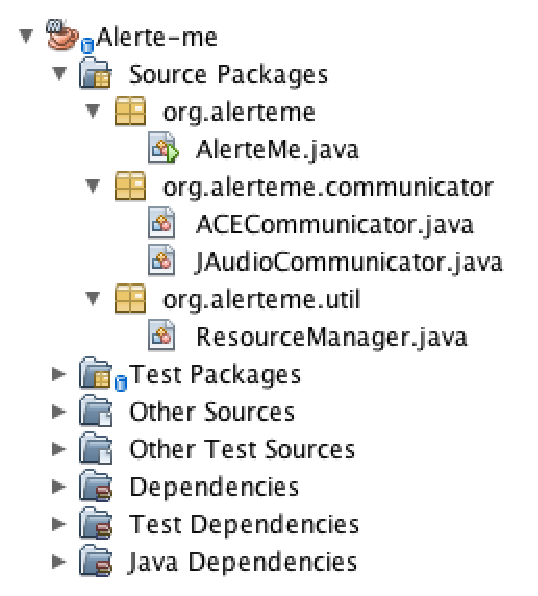
\includegraphics[scale=0.80]{capitulos/validacao/figuras/arquiteturaDoSistemaDesenvolvido.eps}
	\caption{Arquitetura utilizada no sistema desenvolvido}
	\label{fig:result-engajamento}
\end{figure}

Com base na figura podemos ver que o projeto conta com um pacote chamado Communicator, que por sua vez estão presentes as classes ACECommunicator e JAudioCommunicator, responsáveis por executarem suas respectivas ferramentas e se comunicarem com o AlertMe. A classe AlertMe é responsável por chamar todas as classes Communicator e executa-las. O projeto possui um pacote chamado Test, neste pacote estão pacotes e classes com a tarefa de automatizar todos os testes desenvolvidos no AlertMe. 

\section{Processo de automação dos testes}

O processo de automação de testes para o sistema desenvolvido foi organizado com o intuito de unir atividades de desenvolvimento e a qualidade do software gerado em tempo de desenvolvimento e não apenas como uma atividade final de validação. Para que isso fosse possível, as atividades de automação foram conduzidas juntamente com o desenvolvedor, o trabalho foi realizado iterativamente com base no que era criado para o sistema.

\begin{figure}[H]
	\centering
	\captionsetup{justification=centering,margin=2cm}
	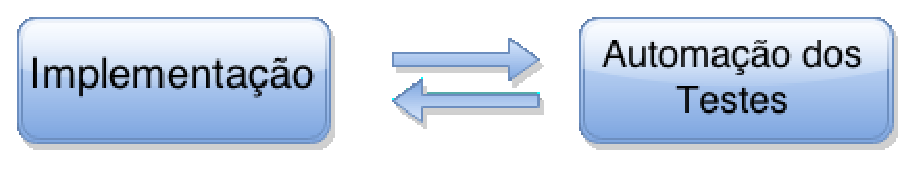
\includegraphics[scale=0.80]{capitulos/validacao/figuras/automationTestProcess.eps}
	\caption{Representação da integração do desenvolvimento e automação dos testes}
	\label{fig:result-engajamento}
\end{figure}

Foi possível observar, que a utilização dessa integração entre desenvolvimento e testes automatizados representou grande impacto na implementação e preocupação na qualidade do código produzido. Toda nova implementação realizada era validada através da automação de novos testes e a reutilização de testes que já tinham sido desenvolvidos, garantindo que essa nova versão ou funcionalidade não quebraria o sistema.

\subsection{Definição dos objetivos dos testes}

Inicialmente, foi conduzida uma análise das ferramentas que iriam compor a arquitetura do projeto: jAudio e ACE. Como elas iriam se integrar dentro da aplicação. Essa análise foi feita a partir de discussões com o desenvolvedor para entender como esses pacotes de softwares funcionavam e de como iriam ser utilizados. Essas conversas serviram muitas vezes como análise da própria arquitetura, antes da implementação e do levantamento dos testes que iriam ser automatizado. Foi possível também identificar que os testes de unidade referente ao jAudio e ACE não fariam parte do escopo deste trabalho, por serem frameworks já testados e que o principal desafio para automação proposta, seria então desenvolver testes automatizados que validassem a integração entres essas ferramentas e o sistema protótipo proposto. Logo, os objetivos da automação dos testes dessa aplicação foram a integração das ferramentas (jAudio e ACE), o funcionamento delas separadamente, mas não a nível de testar os algoritmos utilizados por ambas e sim o que era esperado como reposta da execução dessa integração.

\subsection{Implementação dos testes unitários e integração}

Depois da analise feita para identificação dos objetivos da automação e implementação do sistema, foi desenvolvida duas classes: ACECommunicator e JAudioCommunicator. Estas por sua vez, são as responsáveis por executar as ferramentas ACE e jAudio dentro da aplicação. A seguir serão listados os tipos de automação de testes desenvolvidos para cobertura de níveis unitários e de integração. As classes responsáveis por este nível de testes automatizados encontrasse dentro do pacote Communicator que pertence ao pacote de testes do projeto.  

\begin{figure}[H]
	\centering
	\captionsetup{justification=centering,margin=2cm}
	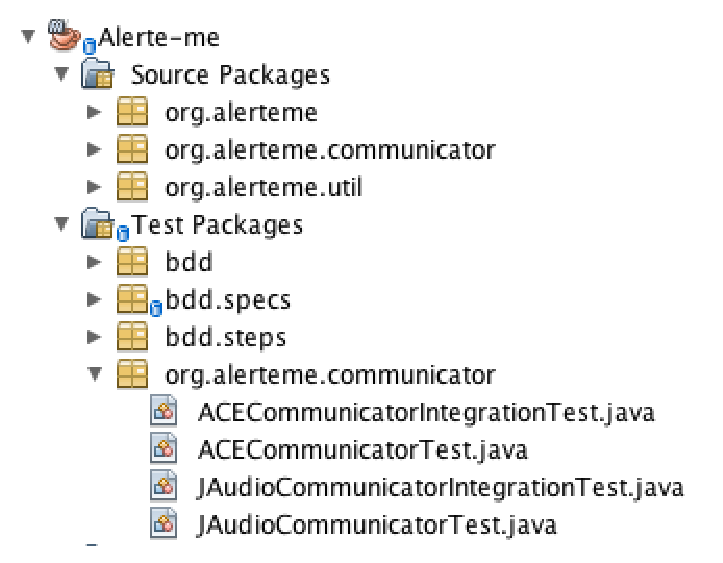
\includegraphics[scale=0.80]{capitulos/validacao/figuras/testesUnitEdIntegra.eps}
	\caption{Arquitetura dos pacotes de testes automatizados de unidade e integração, dentro do pacote de testes Communicator.}
	\label{fig:result-engajamento}
\end{figure}


\begin{itemize}
	\item jAudioCommunicator

Essa classe possui a responsabilidade de extração de características do áudio e como resposta, a criação de um arquivo “output.xml“  que irá conter todas as informações necessárias deste áudio para serem usadas na classificação.  Ela contem um método chamado extractFeatures  que recebe como parâmetro: arquivo de áudio a ser classificado, arquivo settings.xml que possui as configurações que o algoritmo de extração do jAudio necessita e nome do arquivo de output que será preenchido com as características que a extração realizará.  Para que a extração das características e o consequente uso eficaz do jAudio funcione este método precisa validar todos estes argumentos.

Nestas duas primeiras tabelas são apresentados os testes desenvolvidos para validação como unidade do jAudio e estão presentes na classe JAudioCommunicatorTeste.


\begin{figure}[H]
	\centering
	\captionsetup{justification=centering,margin=2cm}
	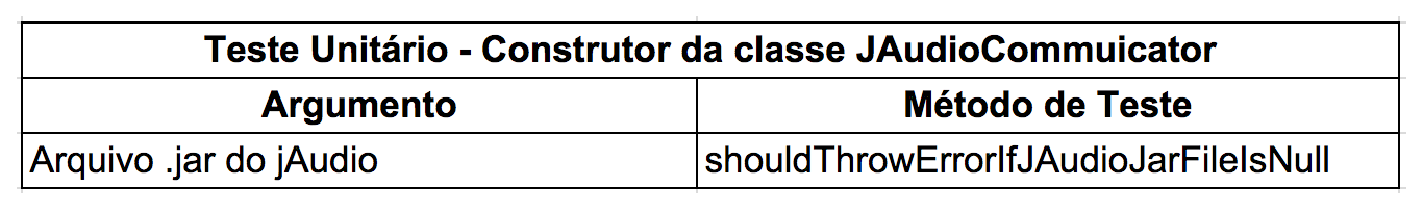
\includegraphics[scale=0.65]{capitulos/validacao/figuras/testeConstrutorJAudioCommunicator.eps}
	\caption{Teste para validação do construtor da classe JAudioCommunicator}
	\label{fig:result-engajamento}
\end{figure}
	
A validação acima garante que caso o sistema não encontre o arquivo ".jar" do jAudio, a aplicação retornará uma mensagem de erro. 

\begin{figure}[H]
	\centering
	\captionsetup{justification=centering,margin=2cm}
	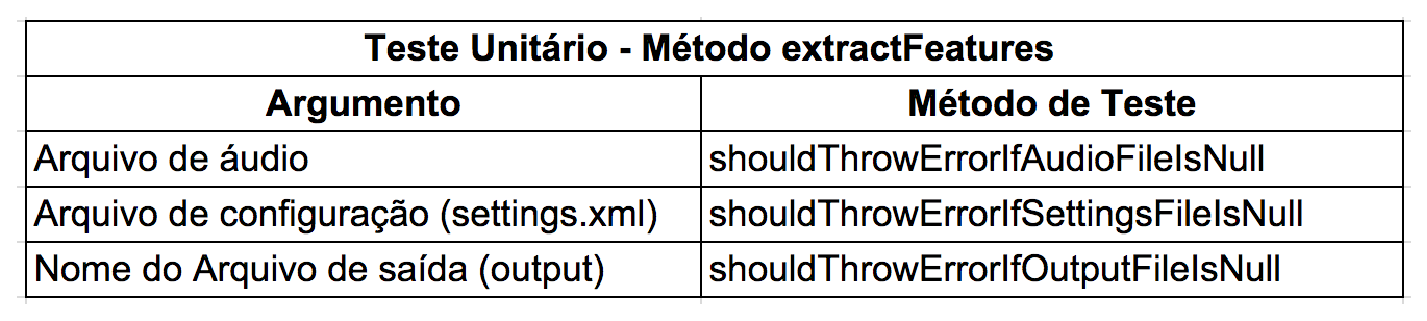
\includegraphics[scale=0.65]{capitulos/validacao/figuras/testeUniJaudioCommunicator.eps}
	\caption{Implementação dos testes unitários para classe JAudioCommunicator}
	\label{fig:result-engajamento}
\end{figure}

Esses testes validam que o arquivo de áudio, arquivo de configuração e o nome do arquivo de saída não são nulos. Todos os testes garantem que caso um destes arquivos não sejam encontrados ou estejam nulos a aplicação retornará uma mensagem facilitando a vida do usuário para entender qual o erro aconteceu e onde aconteceu. 

Como resultado da extração das características do áudio, temos a criação de dois arquivos de output, o outputFeatureVector e o outputFeatureKey. Alguns testes de integração para validação da criação destes arquivos de output foram desenvolvidos:

\begin{figure}[H]
	\centering
	\captionsetup{justification=centering,margin=2cm}
	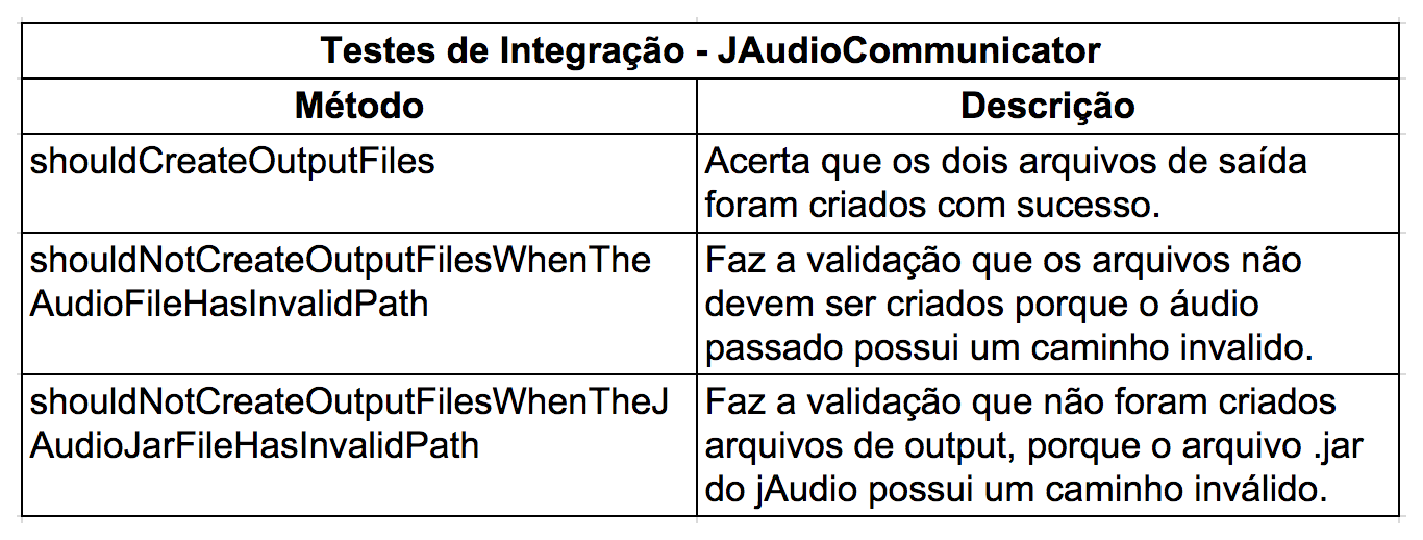
\includegraphics[scale=0.65]{capitulos/validacao/figuras/testesIntegracaoJAudioCommunicator.eps}
	\caption{Implementação dos testes de integração para classe JAudioCommunicator}
	\label{fig:result-engajamento}
\end{figure}
	
Estes testes estão em uma classe chamada JAudioCommunicatorIntegrationTest, pois necessitam de arquivos que servem como entrada para realizar o teste e validar a integração do jAudio com a aplicação. 	
	
	\item ACECommunicator

Esta classe é responsável em executar o ACE e integra-lo com o sistema, é esta classe que possui um método chamado classify, responsável na realização de fato da classificação do arquivo de áudio que foi passado para o jAudio. Para que a realização da classificação ocorra, este método recebe alguns parâmetros. Os parâmetros são: taxonomyFile, featureKeyFile, featureVectorFile, trainedMachineFile.  A figura a seguir mostra uma tabela com os métodos que cobrem a validação destes parâmetros e do arquivo .jar que é passado como argumento do construtor da classe.

\begin{figure}[H]
	\centering
	\captionsetup{justification=centering,margin=2cm}
	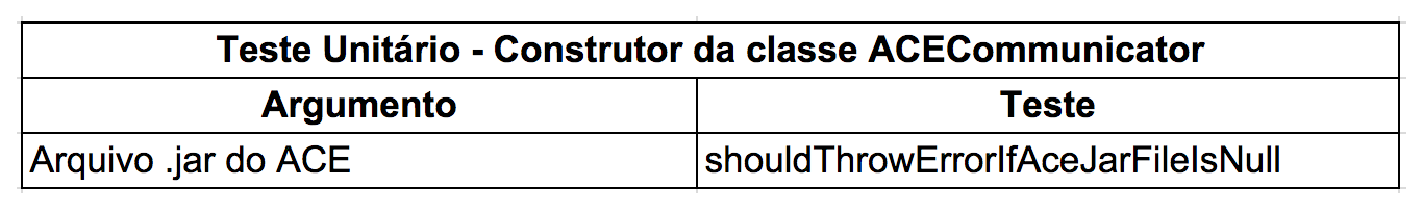
\includegraphics[scale=0.65]{capitulos/validacao/figuras/testeConstrutorACECommunicator.eps}
	\caption{Teste para validação do construtor da classe ACECommunicator}
	\label{fig:result-engajamento}
\end{figure}

Este método de teste garante que caso a classe ACECommunicator não encontre o ".jar" será lançada uma exceção para notificar que o arquivo não foi encontrado.

A seguir são apresentados os testes unitários desenvolvidos para validar o ACECommunicator:

\begin{figure}[H]
	\centering
	\captionsetup{justification=centering,margin=2cm}
	\includegraphics[scale=0.65]{capitulos/validacao/figuras/testeUniACECommunicator.eps}
	\caption{Implementação dos testes unitários para classe ACECommunicator}
	\label{fig:result-engajamento}
\end{figure}

Assim como o JAudioCommunicator, esses testes garantem que caso um  arquivos não sejam encontrados ou estejam nulos a aplicação lançará uma mensagem de erro(exceções) facilitando a vida do usuário e de todo time, no entendimento de qual erro aconteceu e onde aconteceu.

Como resultado da classificação, o ACECommunicator retornará uma lista contendo: o caminho do arquivo de áudio passado e com a resposta da classificação. Para validação desta lista foram criados vários métodos que testam a integração do ACE com a aplicação, testando cenários ,por exemplo, com entradas de arquivos válidos e inválidos. Segue a lista dos métodos de testes de integração desenvolvidos para o ACECommunicator:

\begin{figure}[H]
	\centering
	\captionsetup{justification=centering,margin=2cm}
	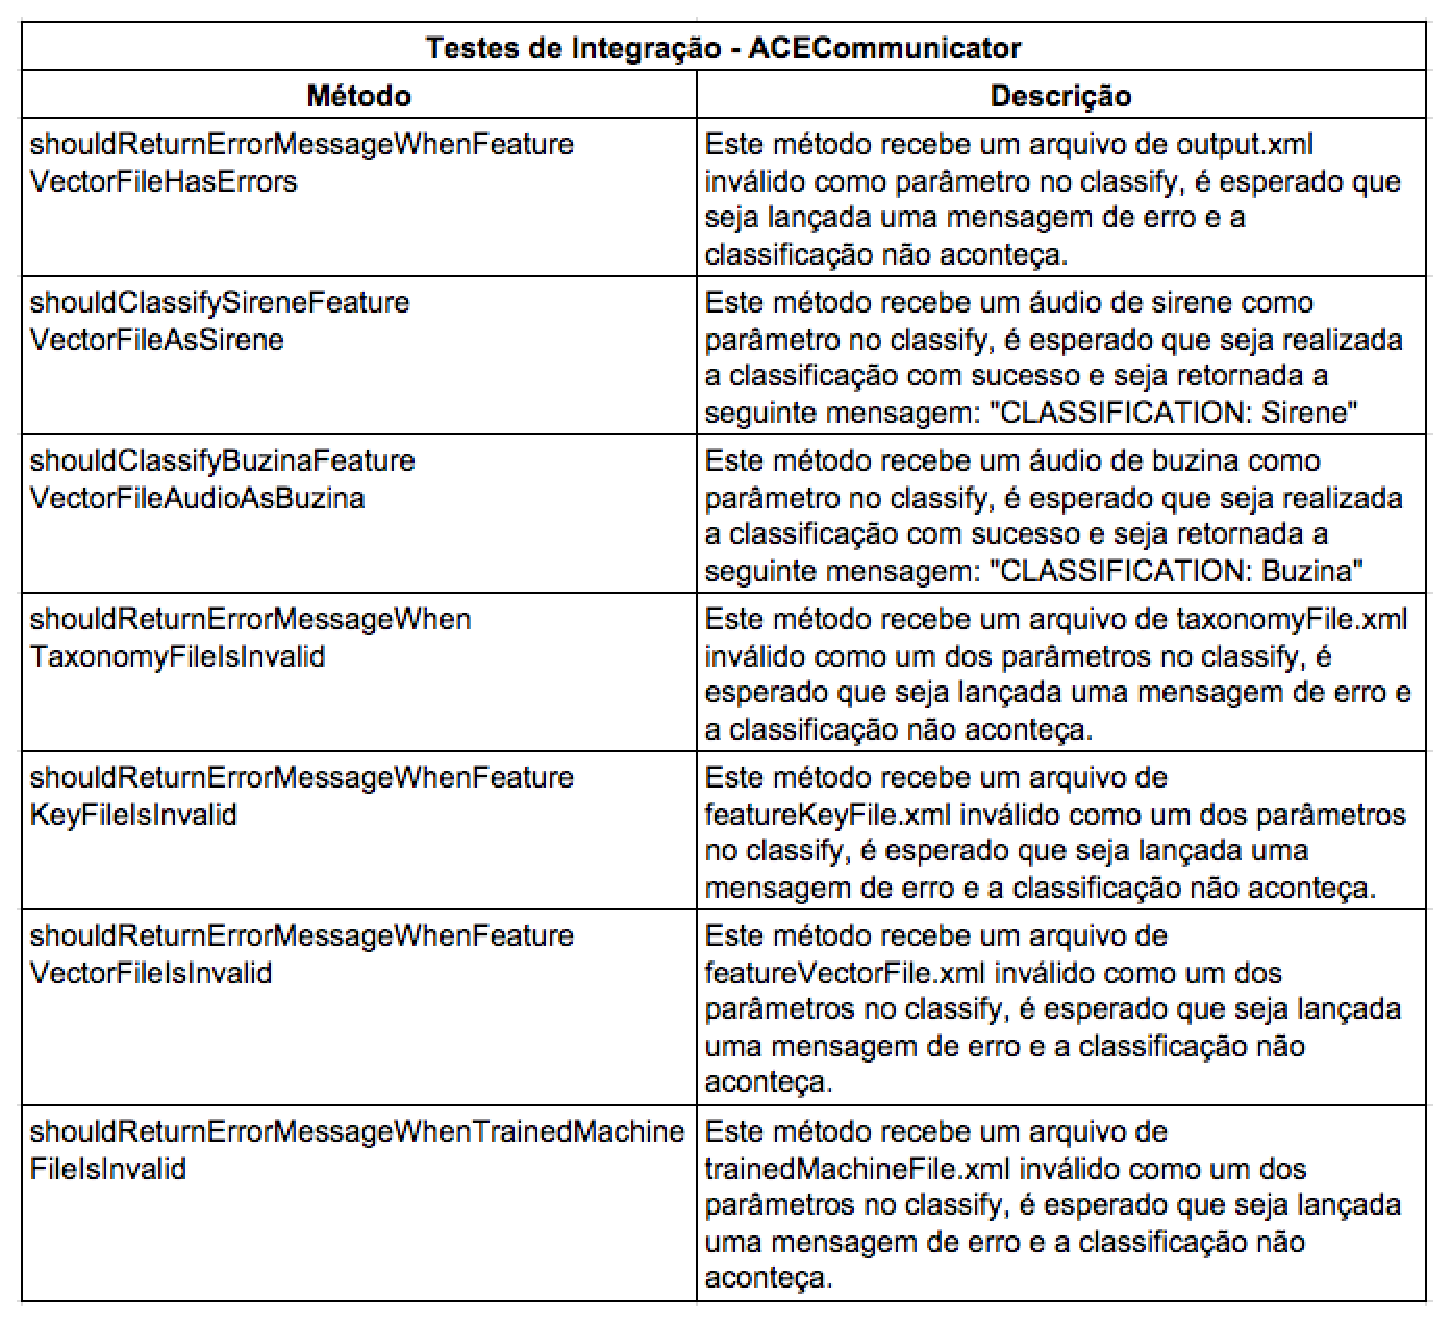
\includegraphics[scale=0.65]{capitulos/validacao/figuras/testesIntegracaoACECommunicator.eps}
	\caption{Implementação dos testes de integração para classe ACECommunicator}
	\label{fig:result-engajamento}
\end{figure}

Os testes de integração da aplicação estão em uma classe chamada ACECommunicatorIntegrationTest, dentro do mesmo pacote estão vários arquivos que foram utilizados como entradas dos cenários de testes.

Um dos métodos, responsável por testar o classify, recebeu um arquivo "invalidOutputFV.xml" (featureVectorFile) inválido como parâmetro no método classify e depois tentou realizar a classificação, mas é esperado que seja feita a validação de uma mensagem de erro para que o time ou usuário entenda porque a classificação não foi realizada com sucesso e qual foi o motivo do insucesso.

\begin{figure}[H]
	\centering
	\captionsetup{justification=centering,margin=2cm}
	\includegraphics[scale=0.55]{capitulos/validacao/figuras/exemploTesteImplementado.eps}
	\caption{Implementação de teste que valida o arquivo featureVectorFile. }
	\label{fig:result-engajamento}
\end{figure}

 Outro método implmentado, utiliza um arquivo xml vindo de um áudio de buzina válido, que foi previamente extraídas suas características com o método extractFeatures pertencente ao JAudioCommunicator, é passado como parâmetro para que o método classify realize a classificação como esperado mostrado a seguir.
 
\begin{figure}[H]
	\centering
	\captionsetup{justification=centering,margin=2cm}
	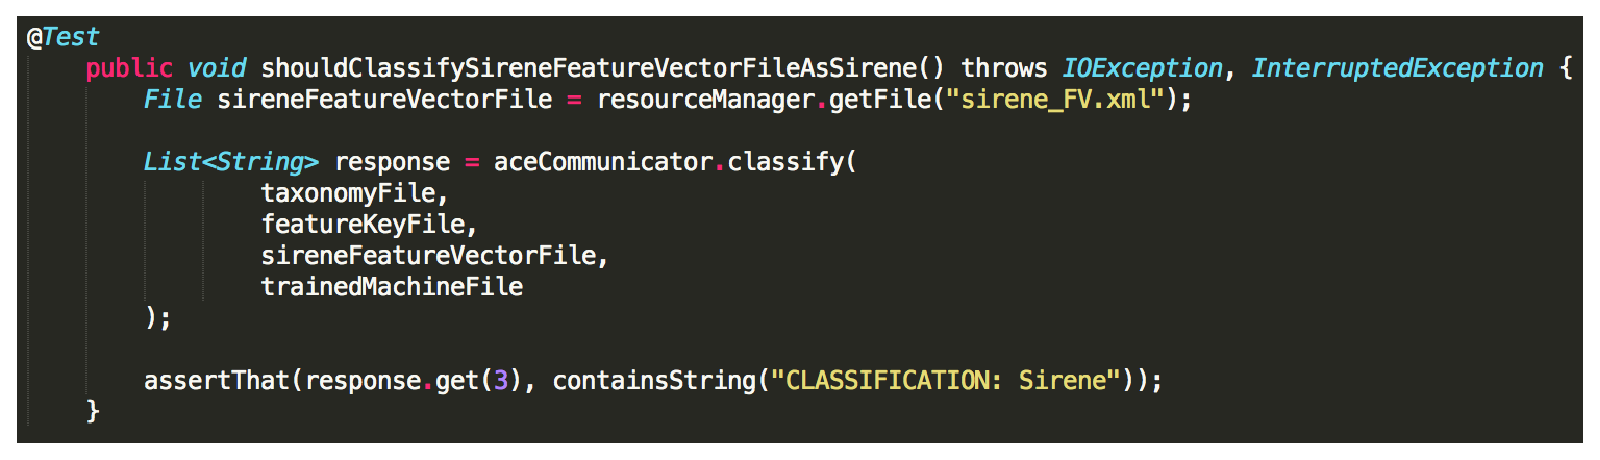
\includegraphics[scale=0.55]{capitulos/validacao/figuras/outroTesteImplementado.eps}
	\caption{Implementação de teste que valida a classificação de um áudio como sirene.}
	\label{fig:result-engajamento}
\end{figure}

\end{itemize}

\subsection{Implementando BDD com Cucumber}

O sistema inicial resultante do desenvolvimento do projeto que este trabalho automatizou os testes não possui interface ainda, mas a ideia protótipo desta interface para smartphone é que seja uma tela simples, com apenas um botão para inserir um áudio e um botão para realizar a classificação, como na ilustração a seguir:


\begin{figure}[H]
	\centering
	\captionsetup{justification=centering,margin=2cm}
	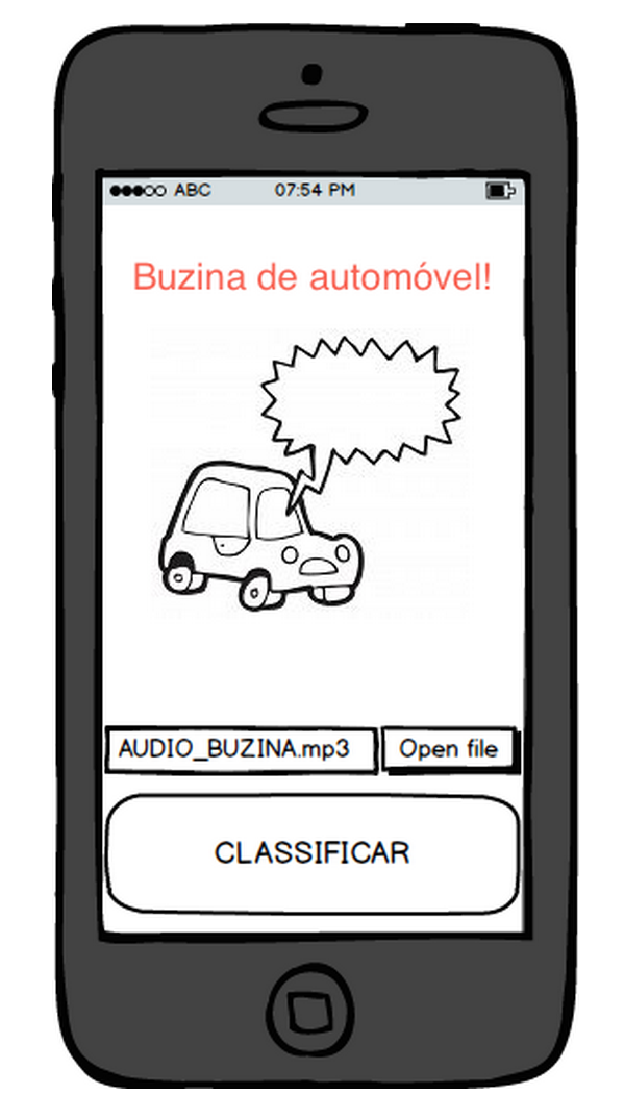
\includegraphics[scale=0.65]{capitulos/validacao/figuras/interfaceDaAplicacao.eps}
	\caption{Protótipo da interface do sistema}
	\label{fig:result-engajamento}
\end{figure}

No inicio da ideação deste projeto uma estória do usuário geral foi criada com intuito de validar a ideia gerada resultante do Brainstorm: 


\begin{figure}[H]
	\centering
	\captionsetup{justification=centering,margin=2cm}
	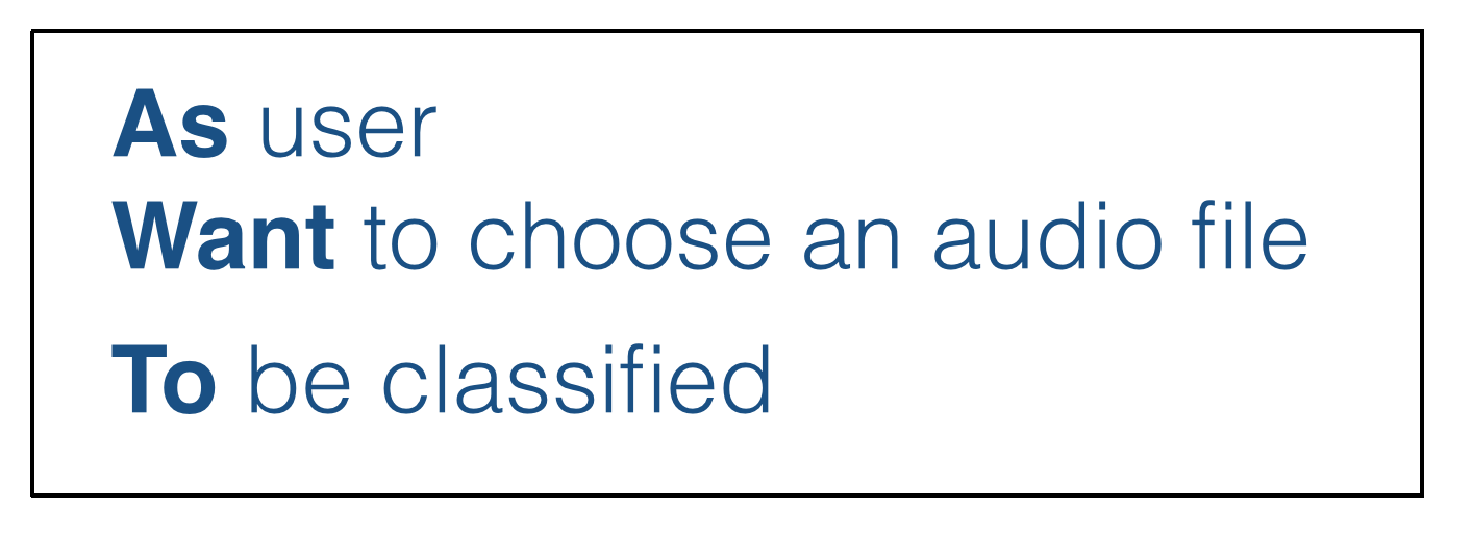
\includegraphics[scale=0.65]{capitulos/validacao/figuras/estoriaDoUsuarioDaAplicacao.eps}
	\caption{Estória do usuário desenvolvida pelo sistema}
	\label{fig:result-engajamento}
\end{figure}

Levando em consideração que o BDD nos permite a análise do comportamento que é esperado do software através da escrita de estórias do usuário com uma linguagem simples e que todos os envolvidos podem entender. Fornecendo cenários para validação do comportamento final, os cenários devem ser criados com base na estória para que validem diversos comportamentos a nível de critérios de aceitação para o cliente ou usuário. Para que a implantação dos testes utilizando BDD com Cucumber fosse possível, dentro do projeto foi criado a arquitetura que o Cucumber entende de pacotes.

\begin{figure}[H]
	\centering
	\captionsetup{justification=centering,margin=2cm}
	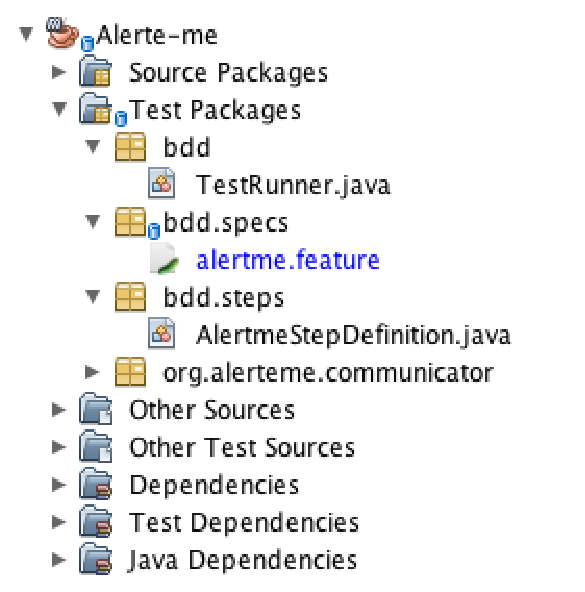
\includegraphics[scale=0.65]{capitulos/validacao/figuras/arquiteturaDeBddComCucumber.eps}
	\caption{Arquitetura dos pacotes responsáveis pela implementação dos testes de BDD com Cucumber.}
	\label{fig:result-engajamento}
\end{figure}

Dentro do pacote bdd, temos outros dois pacotes o specs e os steps. O pacote specs possui os arquivos .features e o steps possui os arquivos que implementam os passos que os cenários descrevem. Ainda na raiz do pacote BDD possuímos a classe java chamada TestRunner.java que é responsável por executar os testes Cucumber.

Foram desenvolvidos três cenários para validar a estória desta aplicação. Como teste de classificação foi usado dois áudios um de buzina e outro de sirene, que serviram para confirmar que a aplicação está realizando a classificação da forma correta. Outro cenário foi a validação de que o sistema reconhece um arquivo passado por parâmetro caso esse seja inválido.


\begin{figure}[H]
	\centering
	\captionsetup{justification=centering,margin=2cm}
	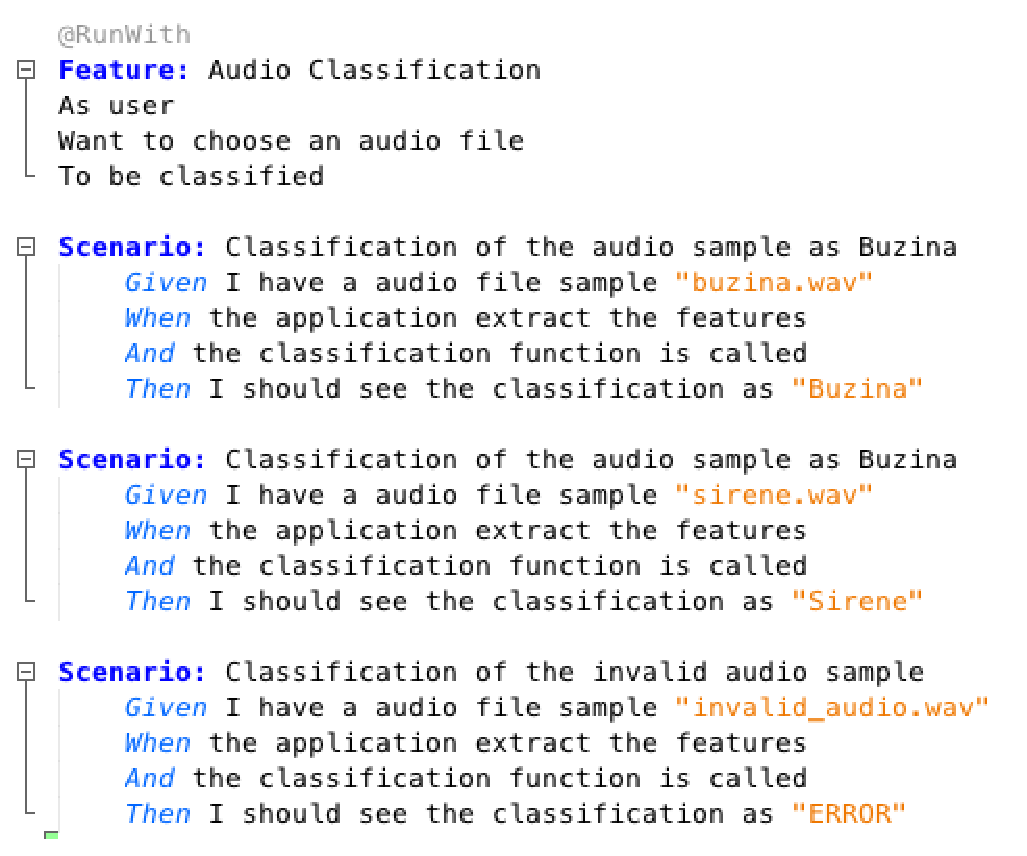
\includegraphics[scale=0.65]{capitulos/validacao/figuras/cenariosDoBDD.eps}
	\caption{Cenários de testes automatizados utilizando Cucumber}
	\label{fig:result-engajamento}
\end{figure}

Para que o Cucumber entenda estes cenários, os steps (passos) que eles possuem devem ser implementados e chamam os métodos responsáveis para que a pré-condição exista e seja validada. A seguir é possível ver a implementação de um dos cenários que foram desenvolvidos:


\begin{figure}[H]
	\centering
	\captionsetup{justification=centering,margin=2cm}
	\includegraphics[scale=0.65]{capitulos/validacao/figuras/implementacaoDeUmStep1.eps}
	\caption{Implementação dos steps de um cenário de teste com Cucumber}
	\label{fig:result-engajamento}
\end{figure}

A seguinte imagem mostra o resultado ao executarmos os cenários de testes, onde são validados e não são encontrados erros:

\begin{figure}[H]
	\centering
	\captionsetup{justification=centering,margin=2cm}
	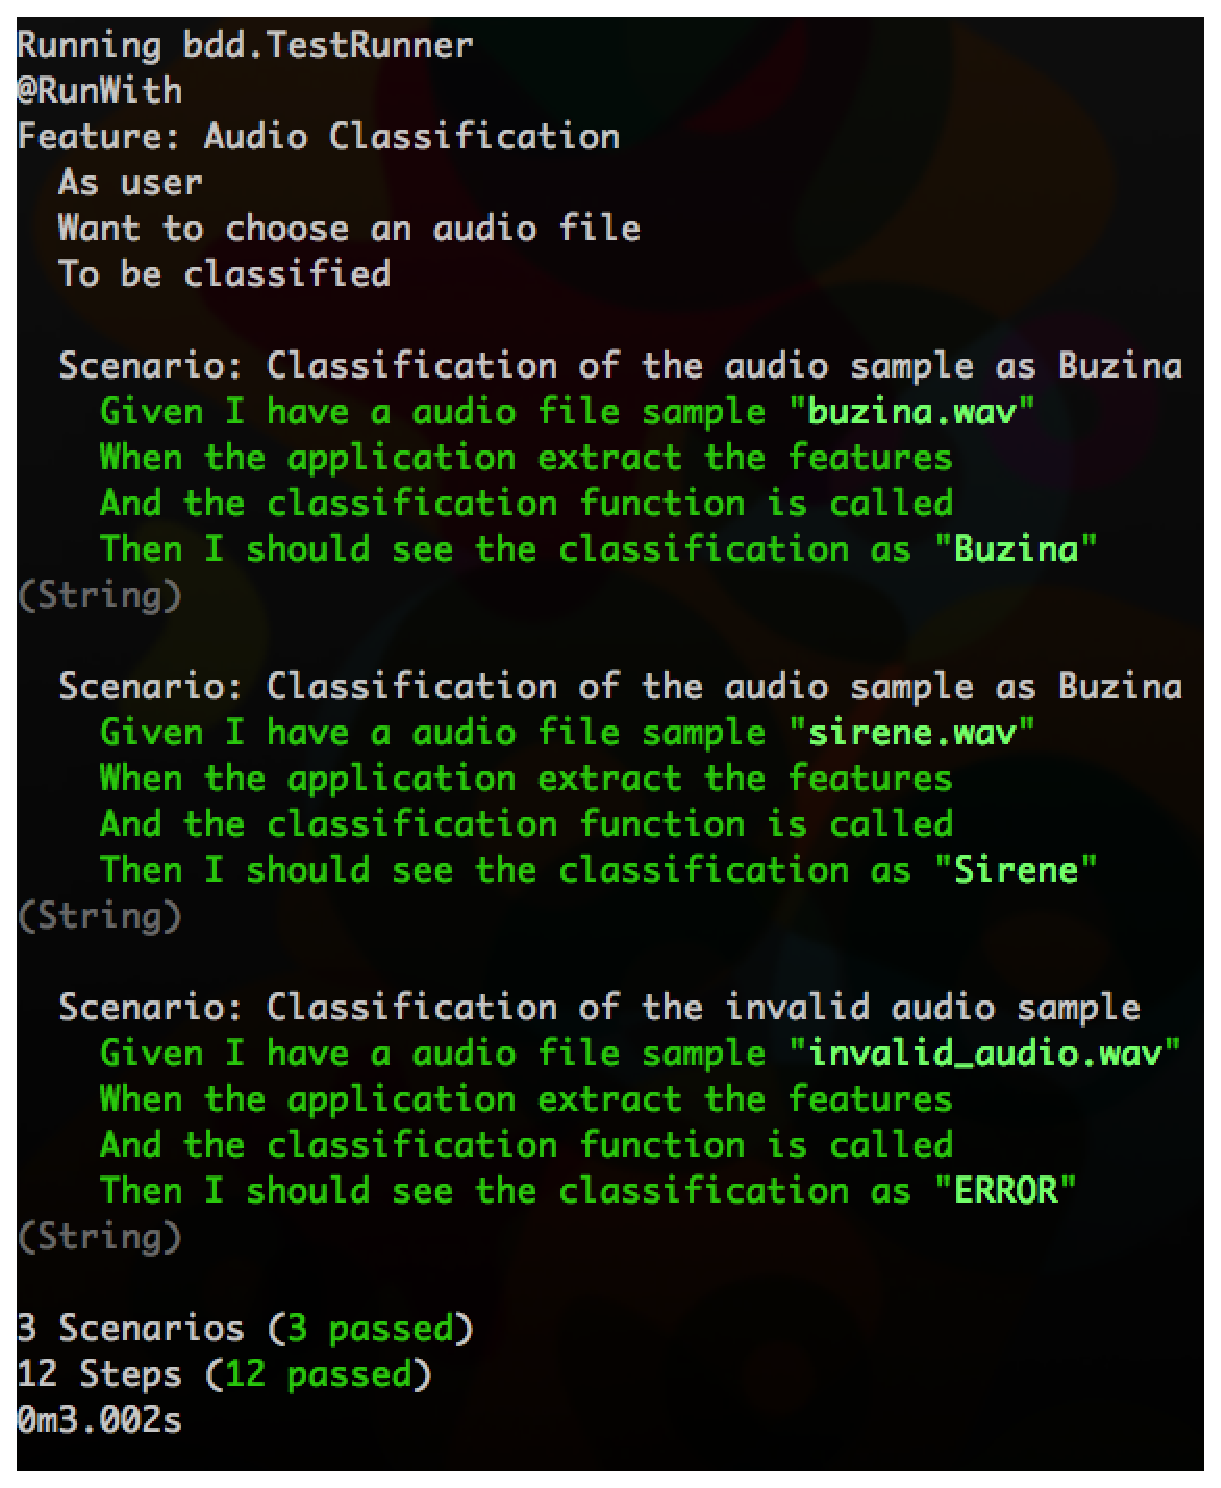
\includegraphics[scale=0.65]{capitulos/validacao/figuras/execucaoDoCucumberEtudoVerde.eps}
	\caption{Resposta da execução dos cenários de testes que foram implementados com Cucumber}
	\label{fig:result-engajamento}
\end{figure}

A figura a seguir é a demonstração de quando um dos cenários não passa ou acontece algum erro na implementação:

\begin{figure}[H]
	\centering
	\captionsetup{justification=centering,margin=2cm}
	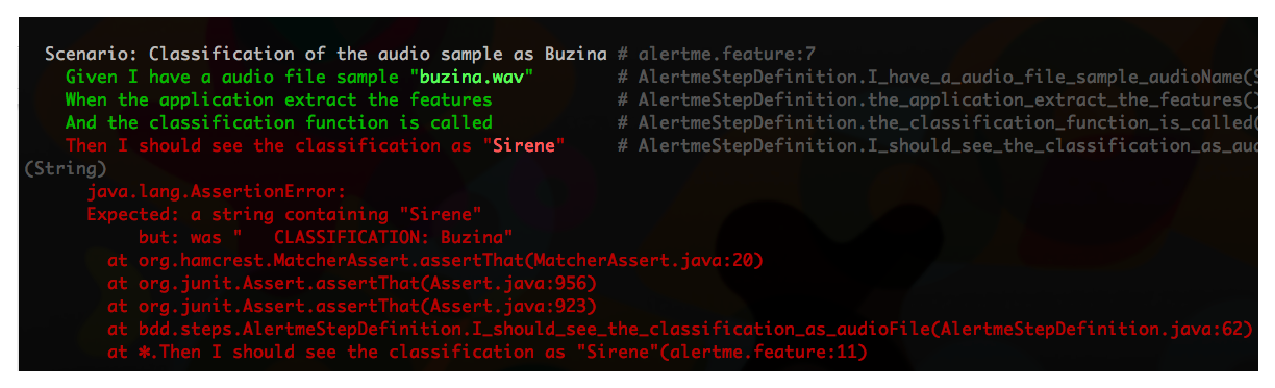
\includegraphics[scale=0.65]{capitulos/validacao/figuras/execucaoDoCucumberComUmErro.eps}
	\caption{Resposta da execução de um cenário de testes que possui um step com falha}
	\label{fig:result-engajamento}
\end{figure}

Este cenário falhou porque era esperado que o resultado da classificação fosse "Sirene" mas a classificação retornou "Buzina". Também como output da execução dos testes automatizados com Cucumber podemos ver o tempo que a execução durou, a quantidade de cenários e testes que falharam ou passaram:

\begin{figure}[H]
	\centering
	\captionsetup{justification=centering,margin=2cm}
	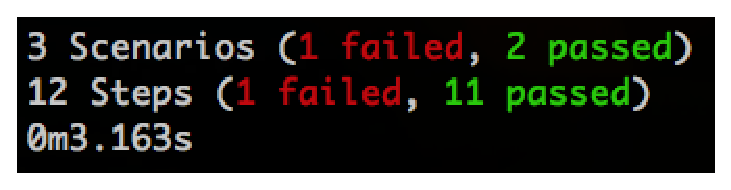
\includegraphics[scale=0.65]{capitulos/validacao/figuras/quantidadeDeErrosQpassaramOUn.eps}
	\caption{Quantidade de cenários de testes e de steps pertencentes a feature executada no Cucumber}
	\label{fig:result-engajamento}
\end{figure}

\section{Resultado da automação dos testes}
Conforme dito previamente este trabalho teve o objetivo de selecionar, implementar e analisar automação de testes durante o desenvolvimento de uma aplicação, para que todo os níveis possíveis da pirâmide de testes \cite{James2011} fossem contemplados com testes automatizados. Como observado na análise dos objetivos da automação, boa parte dos testes foram realizados para validar a integração dos pacotes de software ACE e jAudio com o sistema. O que justifica tomarmos como base para este trabalho a pirâmide a seguir: 

\begin{figure}[H]
	\centering
	\captionsetup{justification=centering,margin=2cm}
	\includegraphics[scale=0.35]{capitulos/validacao/figuras/businesstechnologyautomatedtestingpyramid.eps}
	\caption{Pirâmide de testes dividida nas faces de negócio e tecnologia.}
	\label{fig:result-engajamento}
\end{figure}

Levando em consideração a analise dos objetivos da automação, é visto que esta é a estratégia para aplicação dos testes que melhor se aplica aos resultados que foram coletados ao final deste trabalho.

Para validação da pergunta no topo da pirâmide: "Are we building the right system?" (estamos construindo o sistema certo?), foi realizada a validação com base nos testes de aceitação utilizando BDD com a ferramenta Cucumber,  onde foram desenvolvidos 3 cenários e 12 steps (passos). Este tipo de validação nos ajuda a encontrar divergências entre os principais objetivos do sistema e o seu resultado final esperado, garantindo a verificação do comportamento da aplicação. 

Conforme apresentado na figura, todos os testes de unidade e de integração se encontram na base da pirâmide, respondendo a pergunta: "Are we building the system right?" (Estamos construindo o sistema de forma correta?).  A  aplicação dos testes automatizados, realizados neste trabalho, resultou  em um total de 37 testes, onde 34 destes foram de integração mais unidade e 3 cenários(12 steps) de testes que validam aceitação. É relevante ressaltar que as ferramentas utilizadas ACE e jAudio já possuem uma gama de testes que não fazem parte do escopo desta proposta, mas que ressaltam a importância dos testes que foram realizados serem de integração. Com isso é factível assumir que o desenvolvimento foi coberto por atividades de testes automatizados desde a sua concepção até o final do desenvolvimento. Com praticamente todas as classes e integrações testadas automaticamente ao realizar alguma mudança no projeto e ao gerar um novo build. 

A imagem a seguir mostra a representação da pirâmide resultante deste projeto. 

\begin{figure}[H]
	\centering
	\captionsetup{justification=centering,margin=2cm}
	\includegraphics[scale=0.35]{capitulos/validacao/figuras/pyramid.eps}
	\caption{Pirâmide com as quantidades de testes desenvolvidos neste trabalho}
	\label{fig:result-engajamento}
\end{figure}

